\newpage
\section{Anhang}

\subsection{Trigonometrische Funktionen}
\textcolor{white}{upsi}\\




\begin{minipage}{\linewidth}

\def\colgray{gray}
\def\colblue{blue}
\def\colred{red}
\def\colblack{black}
\renewcommand{\arraystretch}{3.14159265}

\centering

\begin{tabular}{rcccS[table-format=1.4]S[table-format=1.4]}
\toprule
$\displaystyle \varphi$ & $\displaystyle \varphi$ & $\displaystyle \cos \varphi$ & $\displaystyle \sin \varphi$ & \multicolumn{1}{c}{$\displaystyle \cos \varphi$} & \multicolumn{1}{c}{$\displaystyle \sin \varphi$} \\
\midrule
\textcolor{\colblack}{$\displaystyle 0^\circ$} & \textcolor{\colblack}{$\displaystyle 0$} & \textcolor{\colblack}{$\displaystyle 1$} & \textcolor{\colblack}{$\displaystyle 0$} & \multicolumn{1}{c}{\textcolor{\colblack}{1}} & \multicolumn{1}{c}{\textcolor{\colblack}{0}} \\
\midrule
\textcolor{\colgray}{$\displaystyle 15^\circ$} & \textcolor{\colgray}{$\displaystyle \frac{\pi}{12}$} & \textcolor{\colgray}{$\displaystyle \frac{\sqrt{6}+\sqrt{2}}{4}$} & \textcolor{\colgray}{$\displaystyle \frac{\sqrt{6}-\sqrt{2}}{4}$} & \textcolor{\colgray}{0.9659} & \textcolor{\colgray}{0.2588} \\
\textcolor{\colblue}{$\displaystyle 30^\circ$} & \textcolor{\colblue}{$\displaystyle \frac{\pi}{6}$} & \textcolor{\colblue}{$\displaystyle \frac{1}{2}\sqrt{3}$} & \textcolor{\colblue}{$\displaystyle \frac{1}{2}$} & \textcolor{\colblue}{0.866} & \textcolor{\colblue}{0.5} \\
\textcolor{\colred}{$\displaystyle 45^\circ$} & \textcolor{\colred}{$\displaystyle \frac{\pi}{4}$} & \textcolor{\colred}{$\displaystyle \frac{1}{2}\sqrt{2}$} & \textcolor{\colred}{$\displaystyle \frac{1}{2}\sqrt{2}$} & \textcolor{\colred}{0.7071} & \textcolor{\colred}{0.7071} \\
\textcolor{\colblue}{$\displaystyle 60^\circ$} & \textcolor{\colblue}{$\displaystyle \frac{\pi}{3}$} & \textcolor{\colblue}{$\displaystyle \frac{1}{2}$} & \textcolor{\colblue}{$\displaystyle \frac{1}{2}\sqrt{3}$} & \textcolor{\colblue}{0.5} & \textcolor{\colblue}{0.866} \\
\textcolor{\colgray}{$\displaystyle 75^\circ$} & \textcolor{\colgray}{$\displaystyle \frac{5\pi}{12}$} & \textcolor{\colgray}{$\displaystyle \frac{\sqrt{6}-\sqrt{2}}{4}$} & \textcolor{\colgray}{$\displaystyle \frac{\sqrt{6}+\sqrt{2}}{4}$} & \textcolor{\colgray}{0.2588} & \textcolor{\colgray}{0.9659} \\
\midrule
\textcolor{\colblack}{$\displaystyle 90^\circ$} & \textcolor{\colblack}{$\displaystyle \frac{\pi}{2}$} & \textcolor{\colblack}{$\displaystyle 0$} & \textcolor{\colblack}{$\displaystyle 1$} & \multicolumn{1}{c}{\textcolor{\colblack}{0}} & \multicolumn{1}{c}{\textcolor{\colblack}{1}} \\
\midrule
\textcolor{\colgray}{$\displaystyle 105^\circ$} & \textcolor{\colgray}{$\displaystyle \frac{7\pi}{12}$} & \textcolor{\colgray}{$\displaystyle \frac{-\sqrt{6}+\sqrt{2}}{4}$} & \textcolor{\colgray}{$\displaystyle \frac{\sqrt{6}+\sqrt{2}}{4}$} & \textcolor{\colgray}{-0.2588} & \textcolor{\colgray}{0.9659} \\
\textcolor{\colblue}{$\displaystyle 120^\circ$} & \textcolor{\colblue}{$\displaystyle \frac{2\pi}{3}$} & \textcolor{\colblue}{$\displaystyle -\frac{1}{2}$} & \textcolor{\colblue}{$\displaystyle \frac{1}{2}\sqrt{3}$} & \textcolor{\colblue}{-0.5} & \textcolor{\colblue}{0.866} \\
\textcolor{\colred}{$\displaystyle 135^\circ$} & \textcolor{\colred}{$\displaystyle \frac{3\pi}{4}$} & \textcolor{\colred}{$\displaystyle -\frac{1}{2}\sqrt{2}$} & \textcolor{\colred}{$\displaystyle \frac{1}{2}\sqrt{2}$} & \textcolor{\colred}{-0.7071} & \textcolor{\colred}{0.7071} \\
\textcolor{\colblue}{$\displaystyle 150^\circ$} & \textcolor{\colblue}{$\displaystyle \frac{5\pi}{6}$} & \textcolor{\colblue}{$\displaystyle -\frac{1}{2}\sqrt{3}$} & \textcolor{\colblue}{$\displaystyle \frac{1}{2}$} & \textcolor{\colblue}{-0.866} & \textcolor{\colblue}{0.5} \\
\textcolor{\colgray}{$\displaystyle 165^\circ$} & \textcolor{\colgray}{$\displaystyle \frac{11\pi}{12}$} & \textcolor{\colgray}{$\displaystyle \frac{-\sqrt{6}-\sqrt{2}}{4}$} & \textcolor{\colgray}{$\displaystyle \frac{\sqrt{6}-\sqrt{2}}{4}$} & \textcolor{\colgray}{-0.9659} & \textcolor{\colgray}{0.2588} \\
\midrule
\textcolor{\colblack}{$\displaystyle 180^\circ$} & \textcolor{\colblack}{$\displaystyle \pi$} & \textcolor{\colblack}{$\displaystyle -1$} & \textcolor{\colblack}{$\displaystyle 0$} & \multicolumn{1}{c}{\textcolor{\colblack}{-1}} & \multicolumn{1}{c}{\textcolor{\colblack}{0}} \\
\midrule
\textcolor{\colgray}{$\displaystyle 195^\circ$} & \textcolor{\colgray}{$\displaystyle \frac{13\pi}{12}$} & \textcolor{\colgray}{$\displaystyle \frac{-\sqrt{6}-\sqrt{2}}{4}$} & \textcolor{\colgray}{$\displaystyle \frac{-\sqrt{6}+\sqrt{2}}{4}$} & \textcolor{\colgray}{-0.9659} & \textcolor{\colgray}{-0.2588} \\
\textcolor{\colblue}{$\displaystyle 210^\circ$} & \textcolor{\colblue}{$\displaystyle \frac{7\pi}{6}$} & \textcolor{\colblue}{$\displaystyle -\frac{1}{2}\sqrt{3}$} & \textcolor{\colblue}{$\displaystyle -\frac{1}{2}$} & \textcolor{\colblue}{-0.866} & \textcolor{\colblue}{-0.5} \\
\textcolor{\colred}{$\displaystyle 225^\circ$} & \textcolor{\colred}{$\displaystyle \frac{5\pi}{4}$} & \textcolor{\colred}{$\displaystyle -\frac{1}{2}\sqrt{2}$} & \textcolor{\colred}{$\displaystyle -\frac{1}{2}\sqrt{2}$} & \textcolor{\colred}{-0.7071} & \textcolor{\colred}{-0.7071} \\
\textcolor{\colblue}{$\displaystyle 240^\circ$} & \textcolor{\colblue}{$\displaystyle \frac{4\pi}{3}$} & \textcolor{\colblue}{$\displaystyle -\frac{1}{2}$} & \textcolor{\colblue}{$\displaystyle -\frac{1}{2}\sqrt{3}$} & \textcolor{\colblue}{-0.5} & \textcolor{\colblue}{-0.866} \\
\textcolor{\colgray}{$\displaystyle 255^\circ$} & \textcolor{\colgray}{$\displaystyle \frac{17\pi}{12}$} & \textcolor{\colgray}{$\displaystyle \frac{-\sqrt{6}+\sqrt{2}}{4}$} & \textcolor{\colgray}{$\displaystyle \frac{-\sqrt{6}-\sqrt{2}}{4}$} & \textcolor{\colgray}{-0.2588} & \textcolor{\colgray}{-0.9659} \\
\midrule
\textcolor{\colblack}{$\displaystyle 270^\circ$} & \textcolor{\colblack}{$\displaystyle \frac{3\pi}{2}$} & \textcolor{\colblack}{$\displaystyle 0$} & \textcolor{\colblack}{$\displaystyle -1$} & \multicolumn{1}{c}{\textcolor{\colblack}{0}} & \multicolumn{1}{c}{\textcolor{\colblack}{-1}} \\
\midrule
\textcolor{\colgray}{$\displaystyle 285^\circ$} & \textcolor{\colgray}{$\displaystyle \frac{19\pi}{12}$} & \textcolor{\colgray}{$\displaystyle \frac{\sqrt{6}-\sqrt{2}}{4}$} & \textcolor{\colgray}{$\displaystyle \frac{-\sqrt{6}-\sqrt{2}}{4}$} & \textcolor{\colgray}{0.2588} & \textcolor{\colgray}{-0.9659} \\
\textcolor{\colblue}{$\displaystyle 300^\circ$} & \textcolor{\colblue}{$\displaystyle \frac{5\pi}{3}$} & \textcolor{\colblue}{$\displaystyle \frac{1}{2}$} & \textcolor{\colblue}{$\displaystyle -\frac{1}{2}\sqrt{3}$} & \textcolor{\colblue}{0.5} & \textcolor{\colblue}{-0.866} \\
\textcolor{\colred}{$\displaystyle 315^\circ$} & \textcolor{\colred}{$\displaystyle \frac{7\pi}{4}$} & \textcolor{\colred}{$\displaystyle \frac{1}{2}\sqrt{2}$} & \textcolor{\colred}{$\displaystyle -\frac{1}{2}\sqrt{2}$} & \textcolor{\colred}{0.7071} & \textcolor{\colred}{-0.7071} \\
\textcolor{\colblue}{$\displaystyle 330^\circ$} & \textcolor{\colblue}{$\displaystyle \frac{11\pi}{6}$} & \textcolor{\colblue}{$\displaystyle \frac{1}{2}\sqrt{3}$} & \textcolor{\colblue}{$\displaystyle -\frac{1}{2}$} & \textcolor{\colblue}{0.866} & \textcolor{\colblue}{-0.5} \\
\textcolor{\colgray}{$\displaystyle 345^\circ$} & \textcolor{\colgray}{$\displaystyle \frac{23\pi}{12}$} & \textcolor{\colgray}{$\displaystyle \frac{\sqrt{6}+\sqrt{2}}{4}$} & \textcolor{\colgray}{$\displaystyle \frac{-\sqrt{6}+\sqrt{2}}{4}$} & \textcolor{\colgray}{0.9659} & \textcolor{\colgray}{-0.2588} \\
\bottomrule
\end{tabular}

\renewcommand{\arraystretch}{1}
\end{minipage}

\begin{minipage}{.9\textwidth}
  \qquad\qquad
  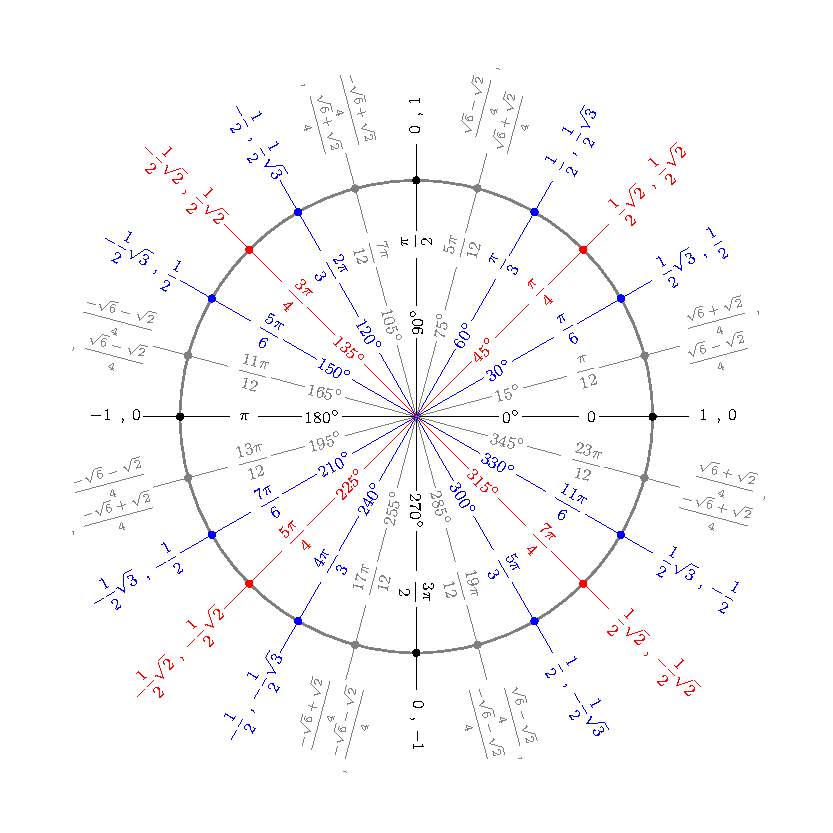
\includegraphics[width=\linewidth]{content/figures/einheitskreis_15}
\end{minipage}



\subsection{Ableitungen}
\textcolor{white}{dupsi}\\

\renewcommand{\arraystretch}{2.718281828}
\begin{tabular}{cccl}
  \toprule
  $f(z)$ & $f'(z)$ & Bereich & Bemerkung \\
  \midrule
  $z^n$ & $n \, z^{n-1}$, $\quad n\in\N$ & $\C$ & \\
  $\quad a_n \, z^n + \cdots + a_1 \, z + a_1 \quad$
   & $\quad n \, a_n \, z^{n-1} + \cdots + 2 \, a_2 \, z + a_1 \quad$
   & $\C$
   & \\
  $\displaystyle\frac{a \, z + b}{c \, z + d}$ & $\displaystyle\frac{ad -bc}{(c \, z + d)^2}$ & $\C\setminus\left\{\frac{-d}{c}\right\}$ & Möbius-Transformation; Ableitung für $f(z)=\infty$ nicht definiert \\
  $e^{az}$ & $a \, e^{az}$ & $\C$ & \\
  $\sin z$ & $\cos z$ & $\C$ & \\
  $\cos z$ & $-\sin z$ & $\C$ & \\
  $\Ln z$ & $\displaystyle\frac{1}{z}$ & $\C \setminus \{ x: x \leq 0 \}$ & \\
  $\sqrt{z}$ & $\displaystyle\frac{1}{2 \sqrt{z}}$ & $\C \setminus \{ x: x \geq 0 \}$ & Positive reelle Achse ansgenommen (anders als im Reellen)! \\
  % $a$ & $a$ & $\C$ & \\
  \bottomrule
\end{tabular}
\renewcommand{\arraystretch}{1}
